\subsection*{Log ind}
Log ind funktionen inddeles i klasser af typen boundary samt en tilhørende controller. Disse fremgår af \autoref{fig:Designlogind}. 

\begin{figure} [H]
\centering
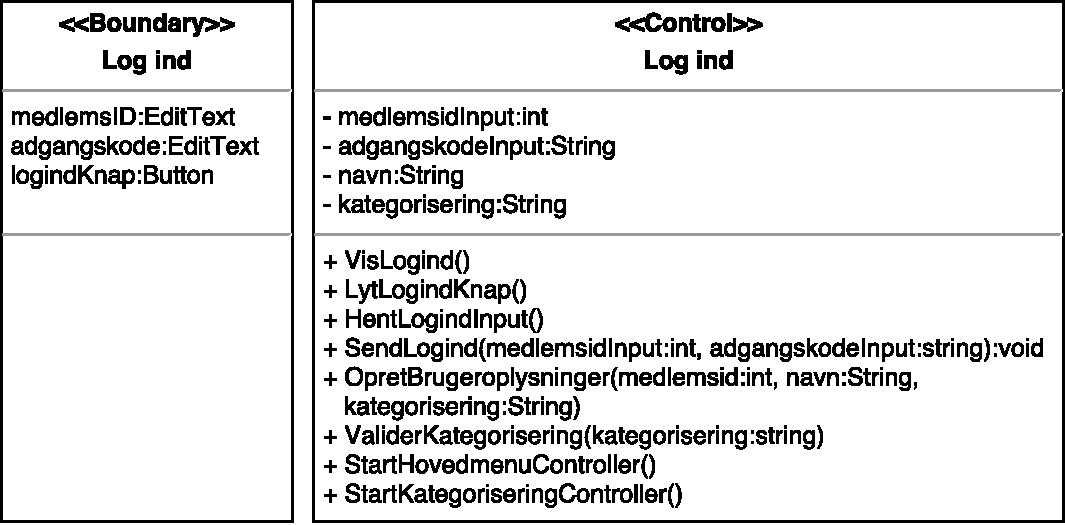
\includegraphics[width=0.9\textwidth]{figures/MVC/MVCLogInd}
\caption{Designklasser for log ind.}
\label{fig:Designlogind}
\end{figure}

\noindent
I grænsefladen for \textit{Logind} opstilles tekstfelter, hvor brugeren kan angive sit medlemsID samt adgangskode. Dertil opsættes en LogindKnap, af typen button, der ved tryk indikerer, at brugerens informationer er angivet og klar til at logge ind. 

Til denne grænseflade er der opstilles en \textit{Logind} controller. Denne controller validerer log ind og opretter tre entity, hvori oplysninger senere kan lagres. Disse entitys ses af \autoref{sec:entity}. Ligeledes håndterer controlleren, hvilken grænseflade systemet efterfølgende skal henvises til. Der er i sammenspil med disse designklasser udarbejdet et sekvensdiagram, der fremgår af \autoref{fig:SEKlogind}.

\begin{figure} [H]
\centering
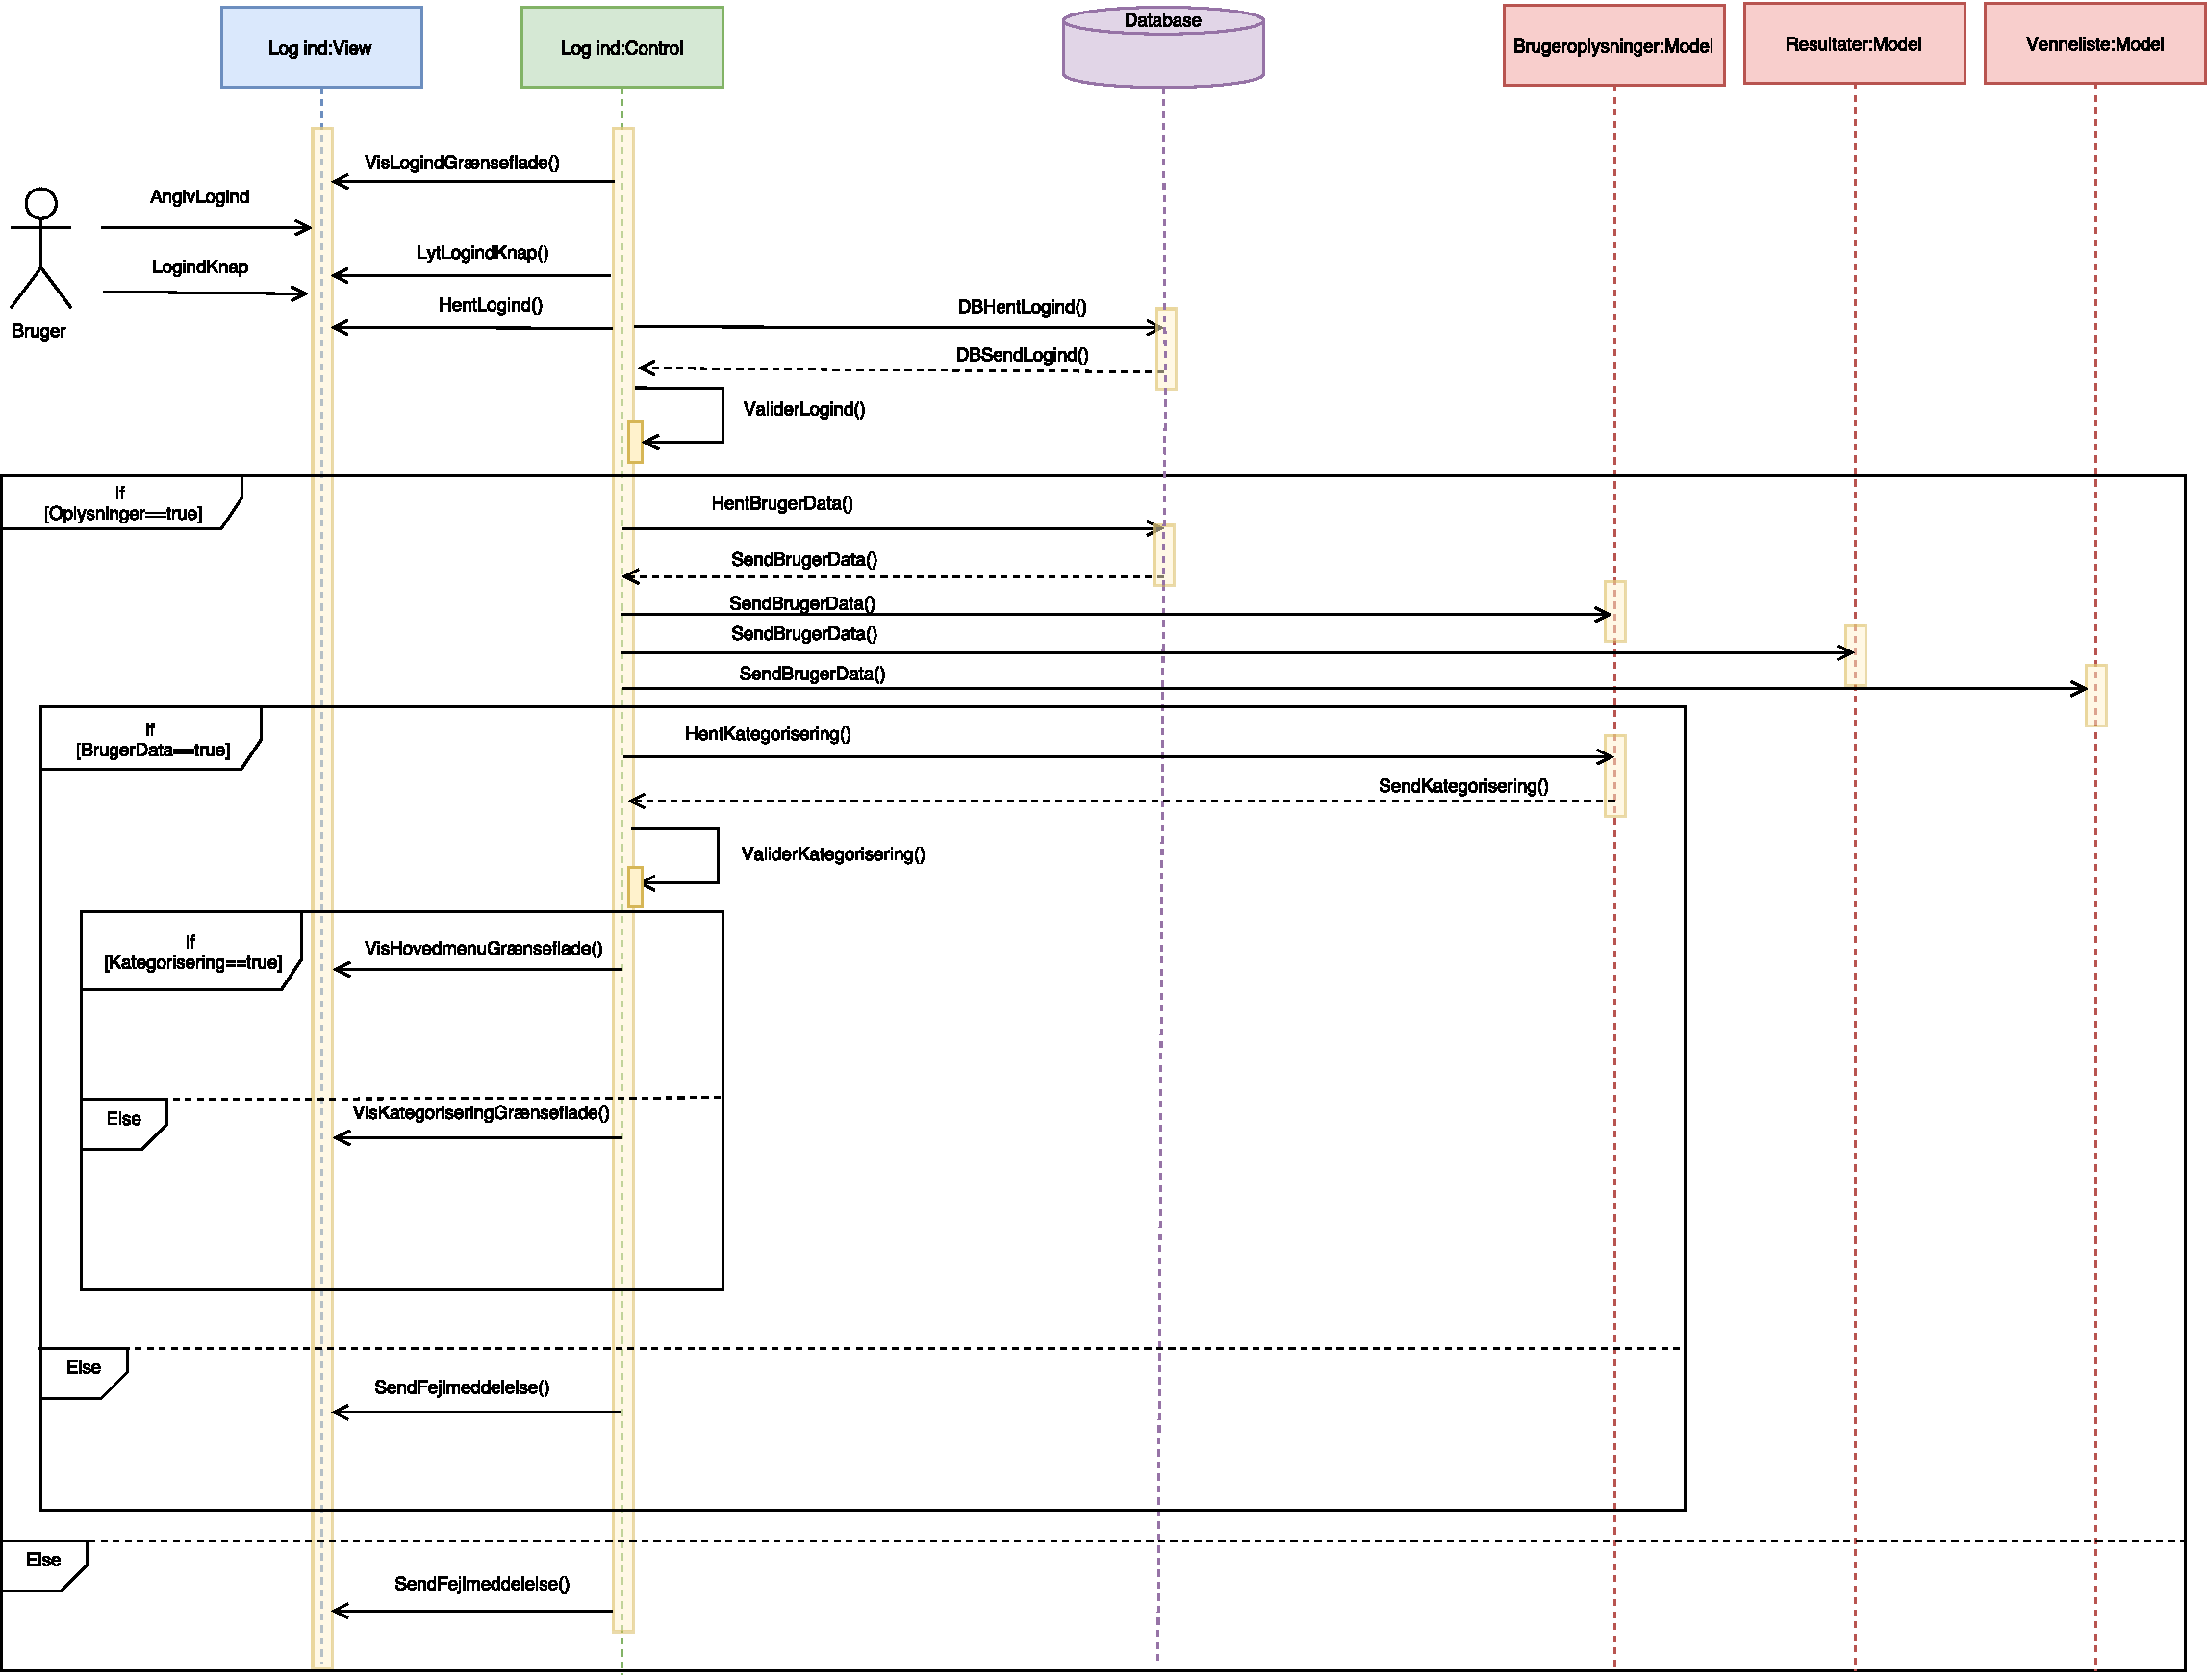
\includegraphics[width=1.1\textwidth]{figures/Sek/SEKLogInd}
\caption{Sekvensdiagram for log ind.}
\label{fig:SEKlogind}
\end{figure}

Det fremgår af dette sekvensdiagram, at controlleren for \textit{Log ind} starter med at vise grænsefladen for \textit{Log ind}. Dertil lytter controlleren på LogindKnap, der ved tryk henter brugerens angivet log ind-informationer. Contolleren henter log ind-informationer passende til det indtastede medlemsID i databasen, hvorefter log ind valideres. Bekræftes log ind oprettes en entity af brugeroplysninger, der henter og lagre brugeroplysninger fra databasen. Forfindes en kategorisering i disse oplysninger, oprettes to yderligere entitys, der omfatter \textit{KonditionResultater} og \textit{Venneliste}. Disse entitys henter og lagrer ligeledes deres respektive data fra databasen. Systemet henvises hertil til hovedmenu, der fremgår af \autoref{fig:SEKhovedmenu}.
Forekommer ingen kategorisering i \textit{Brugeroplysninger}, oprettes de to entitys, \textit{KonditionResultater} og \textit{Venneliste}, dog uden at hente og lagre data fra databasen. Systemet henvises dertil til kategoriseringen, hvilket er illustreret af \autoref{fig:SEKkate}.
Mislykkes log ind vises en fejlmeddelelse til \textit{Log ind} grænsefladen. 
